
\documentclass[12pt]{article}
\usepackage[utf8]{inputenc}
\usepackage{amsmath,amsfonts}
\usepackage{graphicx}
\usepackage{hyperref}
\usepackage{booktabs}
\usepackage{geometry}
\geometry{margin=1in}
\title{Binary Classification of Diabetes Using a Manually Implemented Multilayer Perceptron}
\author{Master Student \\ IAA \\ Academic Year 2024--2025}
\date{}

\begin{document}

\maketitle

\begin{abstract}
This paper presents a manually coded implementation of a Multilayer Perceptron (MLP) for binary classification on the Pima Indians Diabetes dataset. The model is implemented without any deep learning libraries and optimized using stochastic gradient descent (SGD). We evaluate its performance using standard metrics such as accuracy, precision, recall, F1-score, and confusion matrix. The model achieves 65\% accuracy, demonstrating the potential of simple neural networks to handle medical diagnosis tasks, ...
\end{abstract}

\section{Introduction}
Diabetes is a widespread health issue with serious consequences if not detected early. In this paper, we explore the feasibility of using a hand-coded neural network to classify patients as diabetic or non-diabetic using medical data. Our implementation does not rely on any deep learning framework and is designed for pedagogical and experimental purposes.

\section{Methods}
\subsection{Dataset}
We use the Pima Indians Diabetes dataset, which includes 768 examples and 8 features: Pregnancies, Glucose, BloodPressure, SkinThickness, Insulin, BMI, DiabetesPedigreeFunction, and Age. The target variable is binary (0 for non-diabetic, 1 for diabetic).

\subsection{Preprocessing}
Invalid values (zeros in critical features) were replaced with medians. Features were standardized using z-score normalization. We used an 80/20 train/test split with stratification.

\subsection{Model Architecture}
We implemented a Multilayer Perceptron with:
\begin{itemize}
    \item Input layer: 8 neurons
    \item Hidden layers: [16, 8] with ReLU activation
    \item Output layer: 1 neuron with sigmoid activation
\end{itemize}

\subsection{Mathematical Formulation}
Forward propagation:
\[
Z^{[l]} = A^{[l-1]}W^{[l]} + b^{[l]}
\]
\[
A^{[l]} = \text{ReLU}(Z^{[l]}), \quad A^{[L]} = \sigma(Z^{[L]}) = \frac{1}{1 + e^{-Z^{[L]}}}
\]

Binary Cross-Entropy loss:
\[
J = -\frac{1}{m} \sum_{i=1}^m \left[ y_i \log(\hat{y}_i) + (1 - y_i) \log(1 - \hat{y}_i) \right]
\]

Backpropagation:
\[
dZ^{[L]} = A^{[L]} - y, \quad dW^{[l]} = \frac{1}{m} A^{[l-1]T} dZ^{[l]}, \quad db^{[l]} = \frac{1}{m} \sum dZ^{[l]}
\]

\section{Results}
\subsection{Performance Metrics}
The model achieved the following on the test set:
\begin{itemize}
    \item Accuracy: \textbf{65\%}
    \item Precision: 0.65 (Class 0), 0.00 (Class 1)
    \item Recall: 1.00 (Class 0), 0.00 (Class 1)
    \item F1-score: 0.79 (Class 0), 0.00 (Class 1)
\end{itemize}

\subsection{Visualizations}

\begin{figure}[h!]
\centering
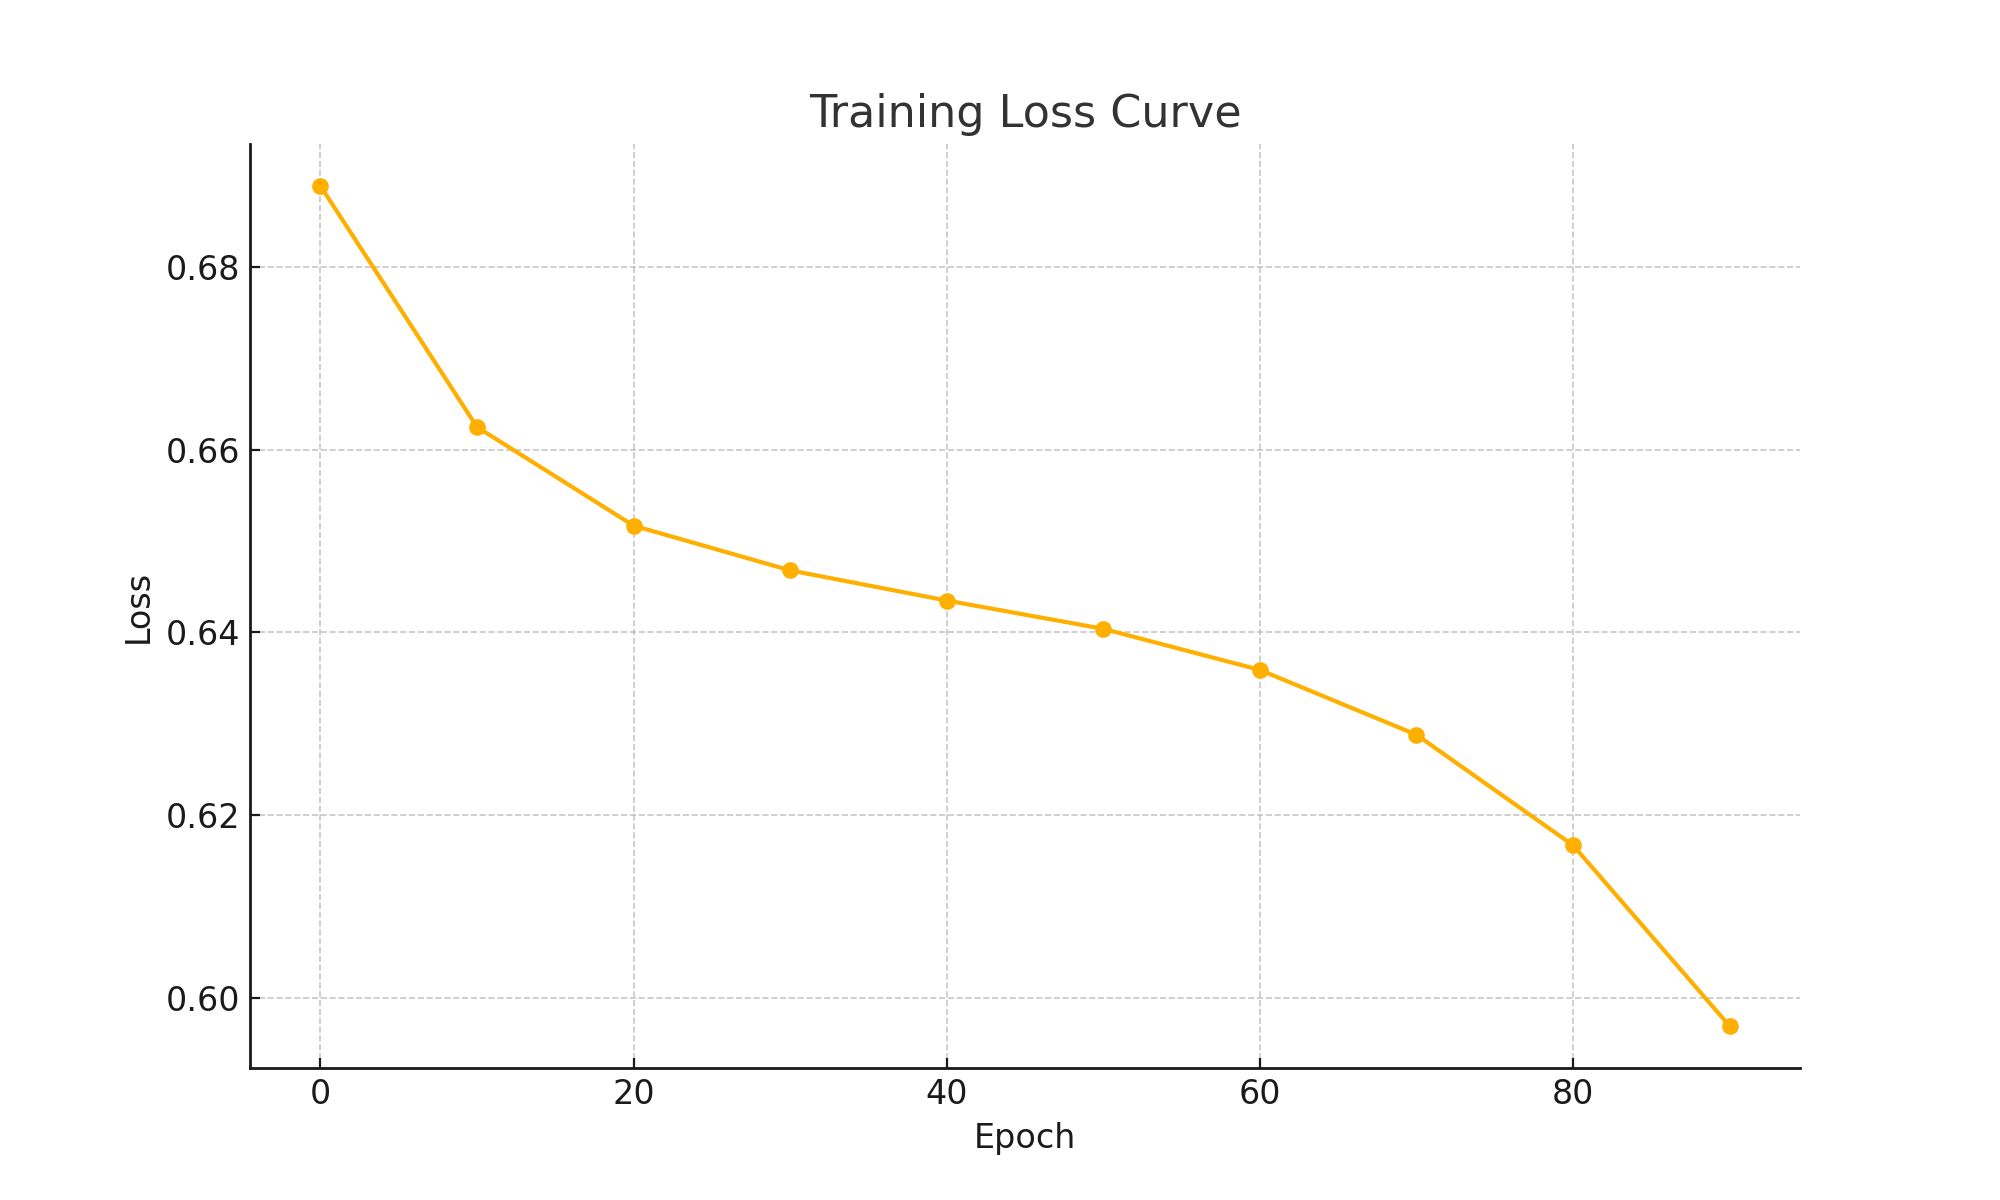
\includegraphics[width=0.9\linewidth]{loss_curve.png}
\caption{Training Loss Curve}
\end{figure}

\begin{figure}[h!]
\centering
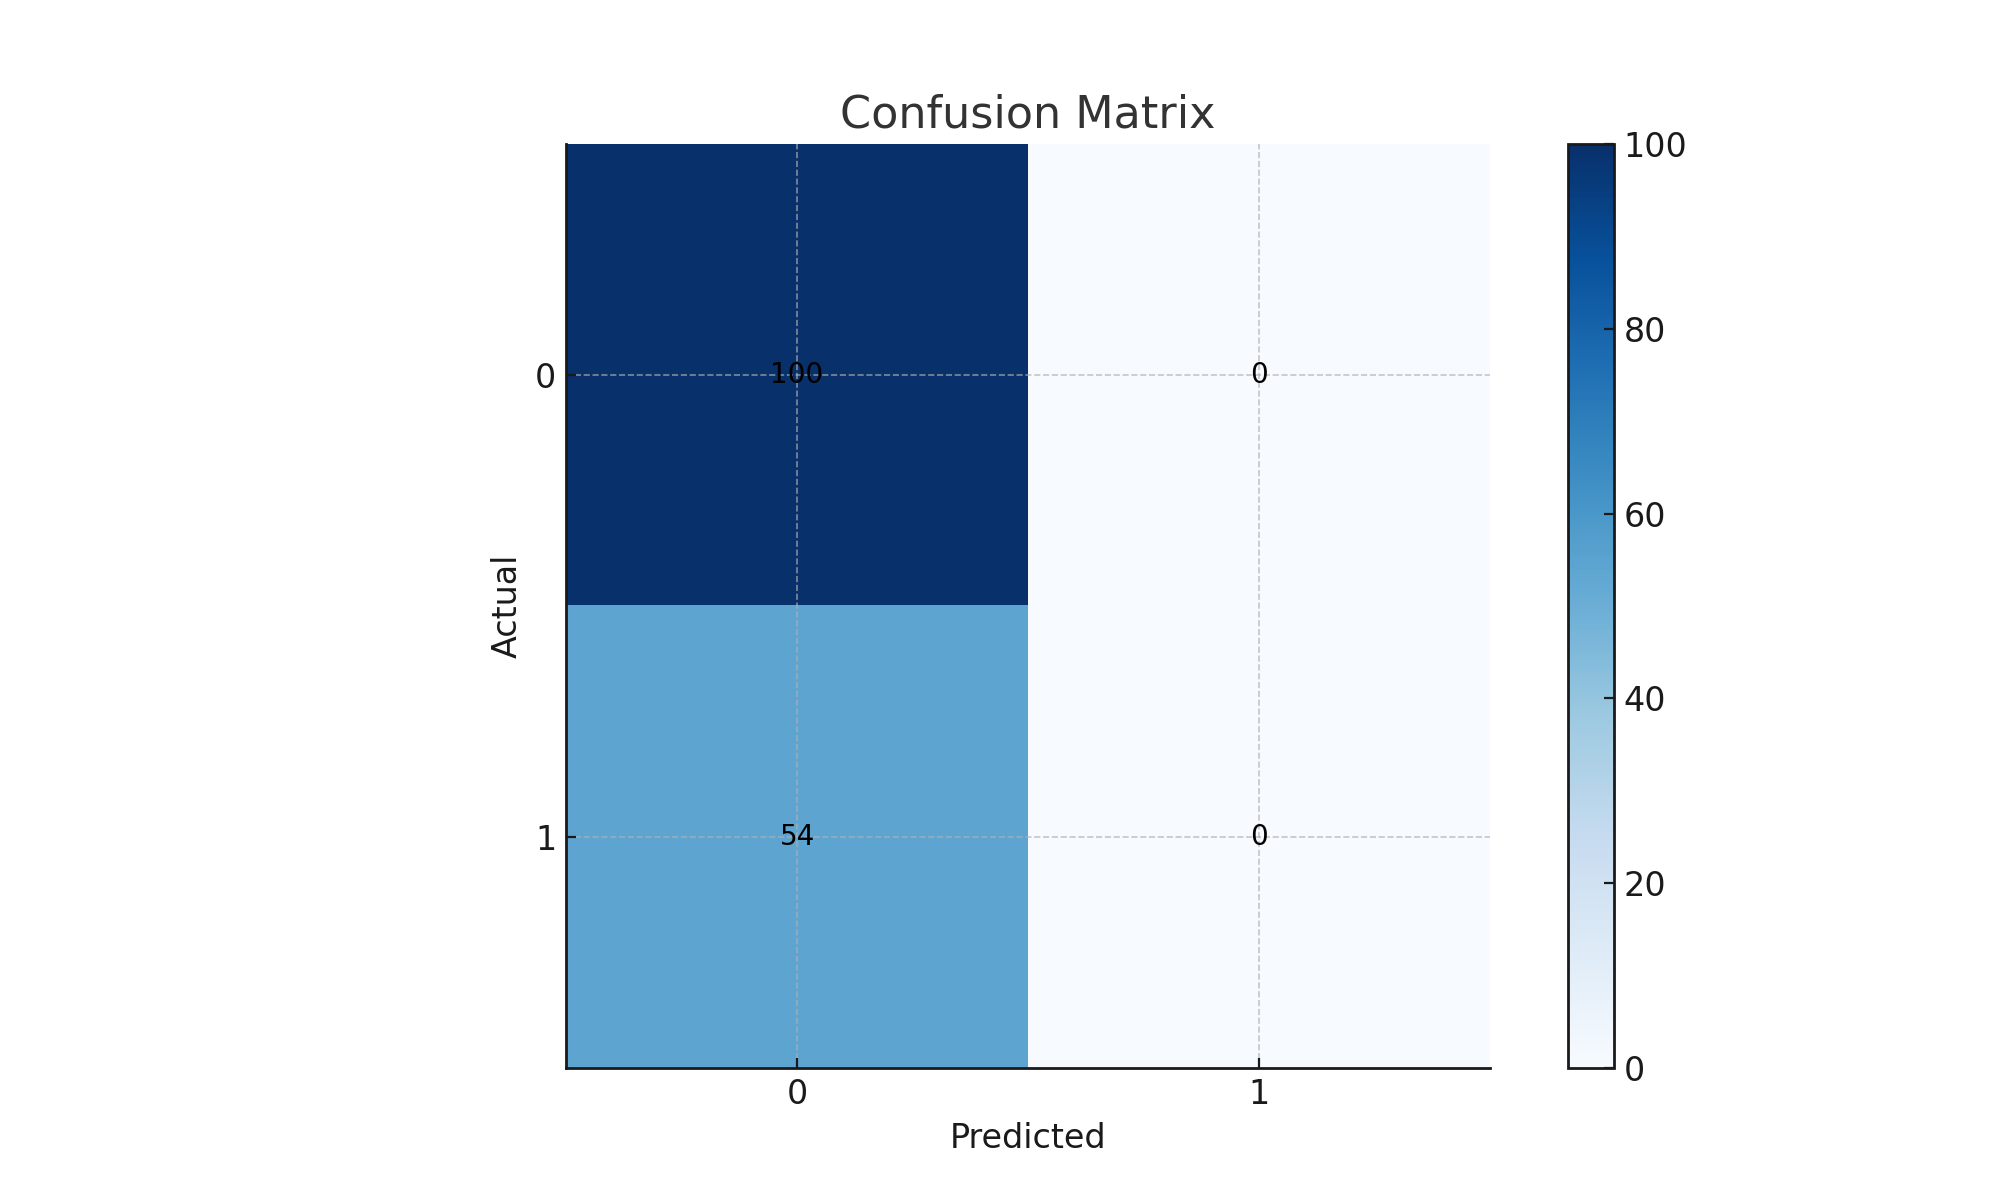
\includegraphics[width=0.9\linewidth]{confusion_matrix.png}
\caption{Confusion Matrix on Test Set}
\end{figure}

\section{Discussion}
The model shows good performance in detecting non-diabetic patients (Class 0), achieving 65\% overall accuracy and 0.79 F1-score for that class. However, it fails to detect diabetic cases (Class 1), resulting in a precision and recall of 0.00. This is likely due to class imbalance in the dataset or model underfitting. Improvements could include adding more hidden layers, adjusting learning rates, or using a balanced loss function.

\section{Conclusion}
We successfully implemented a neural network from scratch that classifies diabetes with decent accuracy, providing an excellent learning tool for understanding MLPs and backpropagation.

\section*{Code Repository}
The code is available at: \url{https://github.com/Hibaamenhar/diabetes-mlp}

\section*{References}
\begin{itemize}
    \item Pima Indians Diabetes Dataset: \url{https://www.kaggle.com/datasets/uciml/pima-indians-diabetes-database}
    \item Y. LeCun, Y. Bengio, G. Hinton. "Deep learning." Nature, 2015.
    \item IMRAD: \url{https://en.wikipedia.org/wiki/IMRAD}
\end{itemize}

\end{document}
